In this study, an agent-based model simulates the pollination of plants in a
forest. The model assumes continuous space and consists of two interacting
agents; \emph{pollinators} and \emph{plants}.  We consider different plant
densities to determine what effect density has on the distribution of pollen.
The plants have a limited supply of pollen that can be gathered by pollinators.
Pollinators in turn transport pollen across the landscape using particular
movement rules during normal foraging.  In this model, movement is determined by
a corrolated random walk.  At each step, pollinators examine the local
neighborhood for plants where they will collect additional pollen and deposit
pollen.

\subsection{Movement}
Movement in the model is centered on the pollinators.  Pollen is carried from
one plant to another.  At each step the movement of a pollinator is conducted in
two stages: \emph{searching} and \emph{movement}.  First, the pollinator checks
a neighborhood of radius $r$ to see if there are any plants within the
neighborhood.  If there are one or more plants, the pollinator chooses the
closest.  If there are two or more that are equidistant from the pollinator, one
is randomly chosen.

If there are no plants within a distance $r$ from the current location of the
pollinator, the pollinators movement is defined using a correlated random walk.
For the correlated random walk, the pollinator chooses a direction based on a
probability distribution in which the higher probabilities are centered about
the their current direction, see \autoref{TurningAngle}.  The pollinator then
takes a step of length between 0 and 1 distributed uniformly in the new chosen
direction.  This length is denoted by $s_j^{(i)}$, which is the $j^{th}-$step
taken by the $i^{th}$ pollinator.

\begin{figure}[h!]
  \begin{center}
    \begin{minipage}[b]{0.48\textwidth}
      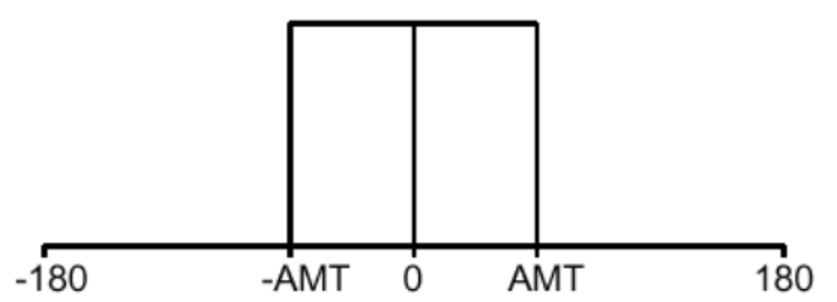
\includegraphics[scale=0.4]{UniformTADistribution.pdf}
      \subcaption{Uniform distribution} \label{sfig:Uniform}
    \end{minipage}
    \begin{minipage}[b]{0.48\textwidth}
      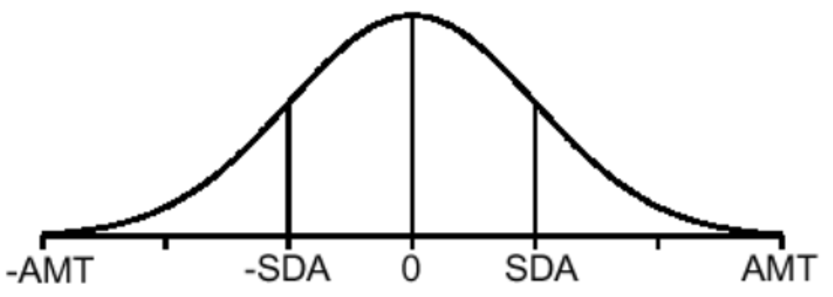
\includegraphics[scale=0.4]{NormalTADistribution.pdf}
      \subcaption{Normal distribution} \label{sfig:Normal}
    \end{minipage}
    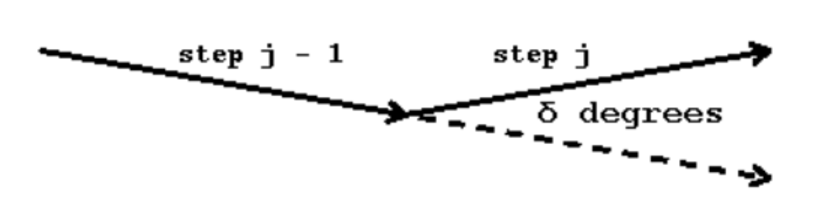
\includegraphics[scale=0.5]{TurningAngle.pdf}
    \subcaption{Example path} \label{sfig:TurningAngle}
  \end{center}
  \caption{Turning Angle for \ref{sfig:Uniform} uniform distribution,
  \ref{sfig:Normal} normal distribution, and \ref{sfig:TurningAngle} depiction
  of what a path may look like.}\label{TurningAngle}
\end{figure}

Alternatively, if the pollinator is already at a plant, the pollinator picks a
random direction uniformly and takes a step of size $r+1.0$.  This will ensure
that the pollinator will not immediately return to the same plant on the very
next step.

\subsection{Pollination}
When an pollinator is on a plant, it collects pollen, distributes pollen, and
consumes food. Each simulated plant contains a number of flowers, $\phi$, from
which an pollinator may obtain pollen. When an pollinator visits a plant it
picks up pollen from one or more flowers. The number of flowers from which an
pollinator can obtain pollen is determined by the total number of flowers on a
plant, the fraction of flowers in bloom at any one time ($a$), the number of
times ($j$) the plant has previously been visited by an pollinator, and the
maximum fraction of flowers available for pollination ($\eta$). The formula for
the number of total flowers available for visitation during a $k^{th}$ visit to
the $j^{th}$ plant ($f_{j,k}$) is given by

\begin{equation}\label{flowers}
f_{j,k} = \phi \cdot a \cdot \eta^k.
\end{equation}

It is assumed that the amount of food eaten and the amount of pollen collected
is proportional to the number of visited flowers. An pollinator collects pollen
and eats from every flower that it visits, and so the amount of pollen collected
and the amount of food eaten is proportional to the equation \eqref{flowers}.
Let $f^{\left(i\right)}_{j,k}$ be the number of flowers visited by the $i^{th}$
pollinator during the $k^{th}$ visit to the $j^{th}$ plant then the amount of
pollen/nectar in the $i^{th}$ pollinator's stomach after $m$ plant visits is
given by

\begin{equation}
c^{\left(i\right)}_m = \sum_{j=0}^{m} \beta f^{\left(i\right)}_{j,k},
\label{limit}
\end{equation}

where $\beta$ is the proportionality constant for the amount of pollen collected
at a plant.  Each pollinator has a maximum amount of food they will ingest,
$c_{max}$, at which time they will stop search for food and return to their
lair. %The total amount of food that an pollinator can eat is limited
%by the stomach size, $c_{max}$.

The fraction, $\alpha$, of all flowers are pollinated, and the associated
probability that a flower is pollinated, $\rho$, are related by the equation,
\begin{equation} \label{Prob} \alpha = \rho \cdot \hat{f}_k.  \end{equation}
Using equation \eqref{limit} and \eqref{Prob} we can determine the probability
that a flower is pollinated, $\rho$, by the formula
\[
  \rho = \frac{\alpha}{\phi} \cdot \frac{1 - \eta}{a \cdot \eta}.
\]

When a flower is pollinated it must determined which previous plant donated the
pollen. Each flower visited is recorded and is available to pollinate the
current flower, except those flowers that are on the same plant. Self-
pollination, is not considered, because the likelihood of self-pollination is
low due to mechanisms that impedes self-pollination. Each flower considered has
an equal likelihood of pollinating the current flower.

\subsection{Time and Stopping Criteria}
The velocity an pollinator travels ($v$) is assumed to be constant, as well as
the time spent on a plant ($t_{plant}$).  The travel time for an pollinator is
then given by the formula
\[
  t^{\left(i\right)} = \frac{s^{\left(i\right)}}{v} + T^{\left(i\right)} \cdot t_{plant},
\]

where $T^{\left(i\right)}$ is the number of plants visited by the $i^{th}$
pollinator. If we let the maximum allowable travel time be $t_{max}$, then once
$t^{\left(i\right)} \geq t_{max}$ or $c^{\left(i\right)}_m \geq c_{max}$ the
pollinator is removed from the simulation. $t_{max}$ is based on the optimal
searching time during the day.  When the pollinator leaves the simulation, it is
terminated.

\subsection{Model Statistics}
To best explore the inherent differences between biotic and abiotic pollination
this study focuses on the effects of movement as well as the effects of plant
density.

\begin{table}[h]
\setlength{\extrarowheight}{1em}
{\tiny
\begin{tabular}{|l|l|}
  \hline
  Measure & Equation \\[8pt] \hline   \hline
  Average Path Distance & $\bar{s} = \frac{1}{b} \sum_{i=1}^b \sum_{j=1}^n s^{\left(i\right)}_j$ \\[8pt] \hline
  Average Maximum Distance & $ \bar{M} = \frac{1}{b} \sum_{i=1}^b \max_j \sqrt{\left(x^{\left(i\right)}_{1,0}
- x^{\left(i\right)}_{1,j}\right)^2 +
      \left(x^{\left(i\right)}_{2,0} -
x^{\left(i\right)}_{2,j}\right)^2}  $ \\[8pt] \hline
  Average Pollination Distance & $ \bar{p} = \frac{1}{n} \sum_{i=1}^{n} \left(
\frac{1}{\tau^{\left(i\right)}} \sum_{j=1}^{\tau^{\left(i\right)}}
\sqrt{\left(x^{\left(i\right)}_1 -
x^{\left(j\right)}_1\right)^2 + \left(x^{\left(i\right)}_2 -
    x^{\left(j\right)}_2\right)^2}
    \right)  $ \\[12pt]  \hline
  Average Maximum Pollination Distance & $ \bar{P} = \frac{1}{n} \sum_{i=1}^{n} \max_j \sqrt{\left(x^{\left(i\right)}_1 -
x^{\left(j\right)}_1\right)^2 + \left(x^{\left(i\right)}_2 -
    x^{\left(j\right)}_2\right)^2}$ \\[8pt]  \hline
  Average Weighted Diversity of Fathers & $ E = \frac{1}{n} \sum_{i=1}^n 1/\frac{1}{\left(\tau^{\left(i\right)}\right)^2}
  \sum_{j=1}^{\Delta\tau^{\left(i\right)}} F^2_{j,i} $ \\[8pt]
  \hline
\end{tabular}
}
\caption{Equations}
\label{tab:eqn}
\end{table}

In order to quantify these way in which the parameters influence the polliation
in this system, we recorded \emph{Average Path Distance} and \emph{Average
Maximum Distance} based upon pollinators directly and \emph{Average Pollination
Distance}, \emph{Average Maximum Pollination Distance}, and \emph{Average
Weighted Diversity of Fathers} based upon the set of pollen that was deposited
at individual plants.  The calculations of these statistics are given in the
\autoref{tab:eqn}.

In these equations it is assumed that $b$ is the number of pollinators, $n$ is
the total number of plants, $(x_{1,0}^{(i)},x_{2,0}^{(i)})$ is the starting
location of the $i^{th}$ pollinator, $(x_{1,j}^{(i)},x_{2,j}^{(i)})$ is the
location of the $i^{th}$ pollinator after $j$ steps, $\tau^{(i)}$ is the total
number of seeds for the $i^{th}$ plant, $\Delta\tau^{(i)}$ is the number of
different fathers contributing pollen to the $i^{th}$ plant, and $F_{j,i}$ is
the number of times the $j^{th}$ father contributed pollen to the $i^{th}$
plant.
